\documentclass[hidelinks,12pt]{article}
\usepackage[left=0.25cm,top=1cm,right=0.25cm,bottom=1cm]{geometry}
%\usepackage[landscape]{geometry}
\textwidth = 20cm
\hoffset = -1cm
\usepackage[utf8]{inputenc}
\usepackage[spanish,es-tabla]{babel}
\usepackage[autostyle,spanish=mexican]{csquotes}
\usepackage[tbtags]{amsmath}
\usepackage{nccmath}
\usepackage{amsthm}
\usepackage{amssymb}
\usepackage{mathrsfs}
\usepackage{graphicx}
\usepackage{subfig}
\usepackage{standalone}
\usepackage[outdir=./Imagenes/]{epstopdf}
\usepackage{siunitx}
\usepackage{physics}
\usepackage{color}
\usepackage{float}
\usepackage{hyperref}
\usepackage{multicol}
%\usepackage{milista}
\usepackage{anyfontsize}
\usepackage{anysize}
%\usepackage{enumerate}
\usepackage[shortlabels]{enumitem}
\usepackage{capt-of}
\usepackage{bm}
\usepackage{relsize}
\usepackage{placeins}
\usepackage{empheq}
\usepackage{cancel}
\usepackage{wrapfig}
\usepackage[flushleft]{threeparttable}
\usepackage{makecell}
\usepackage{fancyhdr}
\usepackage{tikz}
\usepackage{bigints}
\usepackage{scalerel}
\usepackage{pgfplots}
\usepackage{pdflscape}
\pgfplotsset{compat=1.16}
\spanishdecimal{.}
\renewcommand{\baselinestretch}{1.5} 
\renewcommand\labelenumii{\theenumi.{\arabic{enumii}})}
\newcommand{\ptilde}[1]{\ensuremath{{#1}^{\prime}}}
\newcommand{\stilde}[1]{\ensuremath{{#1}^{\prime \prime}}}
\newcommand{\ttilde}[1]{\ensuremath{{#1}^{\prime \prime \prime}}}
\newcommand{\ntilde}[2]{\ensuremath{{#1}^{(#2)}}}

\newtheorem{defi}{{\it Definición}}[section]
\newtheorem{teo}{{\it Teorema}}[section]
\newtheorem{ejemplo}{{\it Ejemplo}}[section]
\newtheorem{propiedad}{{\it Propiedad}}[section]
\newtheorem{lema}{{\it Lema}}[section]
\newtheorem{cor}{Corolario}
\newtheorem{ejer}{Ejercicio}[section]

\newlist{milista}{enumerate}{2}
\setlist[milista,1]{label=\arabic*)}
\setlist[milista,2]{label=\arabic{milistai}.\arabic*)}
\newlength{\depthofsumsign}
\setlength{\depthofsumsign}{\depthof{$\sum$}}
\newcommand{\nsum}[1][1.4]{% only for \displaystyle
    \mathop{%
        \raisebox
            {-#1\depthofsumsign+1\depthofsumsign}
            {\scalebox
                {#1}
                {$\displaystyle\sum$}%
            }
    }
}
\def\scaleint#1{\vcenter{\hbox{\scaleto[3ex]{\displaystyle\int}{#1}}}}
\def\bs{\mkern-12mu}


\title{Segunda solución linealmente independiente} \vspace{-3ex}
\author{M. en C. Gustavo Contreras Mayén}
\date{ }
%s\newcommand{\Cancel}[2][black]{{\color{#1}\cancel{\color{black}#2}}}
\begin{document}
\vspace{-4cm}
\maketitle
\fontsize{14}{14}\selectfont
\tableofcontents
\newpage

\section{Introducción.}

En física a menudo nos encontramos con fenómenos donde se involucra el concepto de un pulso de duración \enquote{infinitamente corto}.
\par
Por ejemplo, en el curso de Mecánica Vectorial se revisó el concepto de una magnitud física llamada \emph{impulso}, la cual se introduce cuando se cambia el estado de movimiento de un cuerpo al aplicarle un \enquote{golpe repentino}. El impulso se denota comúnmente con la letra $I$.
\par
Tomemos como ejemplo del fútbol con un penalty, en este caso tenemos inicialmente al balón en reposo, la intención es que el tirador meta la pelota en la portería contraria. Después de patear el balón, éste adquiere un momento que es igual al impulso asociado a la patada misma. Analíticamente esta afirmación se escribe como
\begin{align*}
m \, v = I = \int_{t_{0}}^{t_{0} + \tau} F(t) \dd{t}
\end{align*}

donde $F(t)$ es la fuerza y $\tau$ la duración del impacto sobre la pelota (técnicamente de la acción de la fuerza sobre el balón).
\par
El término \enquote{repentino} implica que $\tau$ se considera infinitamente pequeño y por tanto, que el cambio en el momento ocurre instantáneamente. Sin embargo, dado que el cambio en el momento es un número finito, se sigue que la magnitud de la fuerza $F(t)$ debió haber sido infinita durante el golpe al balón y cero en cualquier otro momento. Este
tipo de descripciones no se puede formular apropiadamente con los conceptos matemáticos que conocemos, más aún, la descripción tampoco es rigurosa desde un punto de vista físico.
\begin{figure}[H]
    \centering
    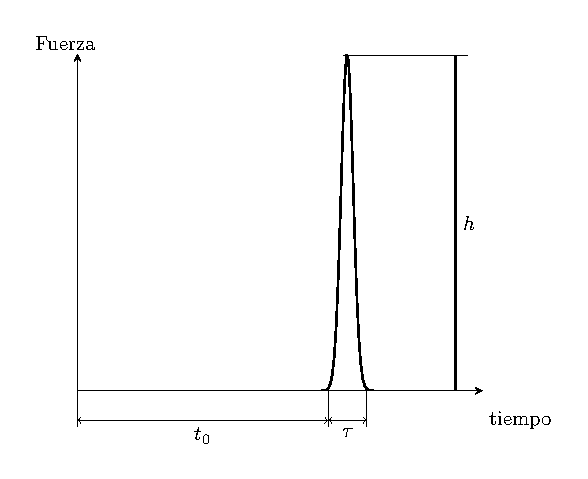
\includegraphics[scale=1]{Imagenes/delta_Dirac_01.eps}
    \caption{Representación del pico para la función.}
    \label{fig:figura_delta_Dirac_01}
\end{figure}

En realidad, la gráfica de la fuerza es una curva muy \enquote{picuda}: muy estrecha y muy alta, como se aprecia en la figura (\ref{fig:figura_delta_Dirac_01}) y satisface la propiedad que el área bajo la curva es igual a $I$. En la gran mayoría de los problemas físicos, la forma exacta de la gráfica no se conoce, sin embargo, en lo correspondiente a los efectos físicos observables asociados con tal función, usualmente esta falta de información no importa. Lo que tiene significado es la integral de la fuerza, esto es, el valor del impulso:
\begin{align*}
I = \int_{t_{0}}^{t_{0} + \tau } F(t) \dd{t}
\end{align*}

Las funciones puntiagudas son comunes en cualquier área de la física, por ejemplo: una fuerza concentrada sobre una barra, es una distribución puntiaguda de la carga, ver la figura (\ref{fig:figura_delta_Dirac_02}). 
\begin{figure}[H]
    \centering
    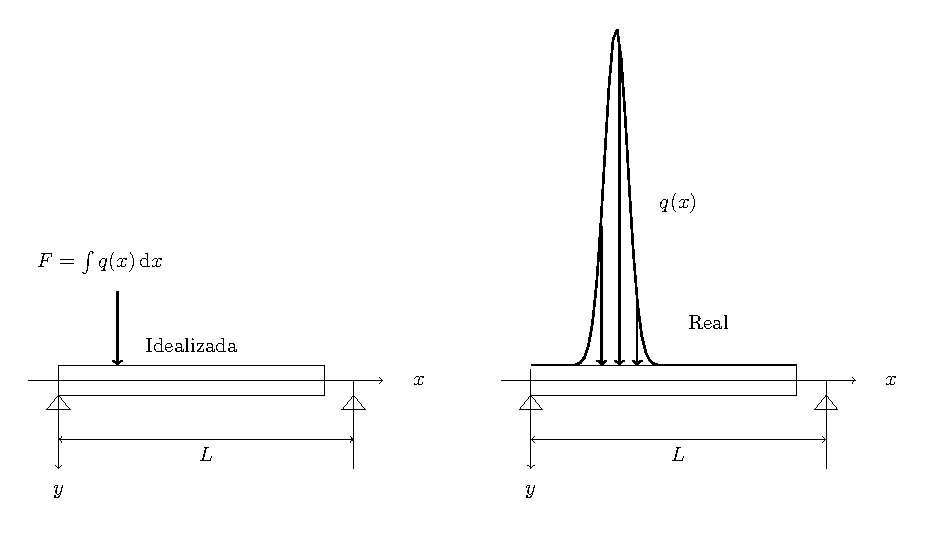
\includegraphics[scale=1]{Imagenes/delta_Dirac_02.eps}
    \caption{Representación de una fuerza aplicada de manera ideal contra la real.}
    \label{fig:figura_delta_Dirac_02}
\end{figure}

En los circuitos eléctricos, las corrientes \enquote{puntiagudas} de una duración extremadamente corta, se presentan cuando se conecta el interruptor, como en el caso de la redistribución de carga entre dos condensadores, como se ve en la figura (\ref{fig_figura_delta_Dirac_03}).
\begin{figure}[H]
    \centering
    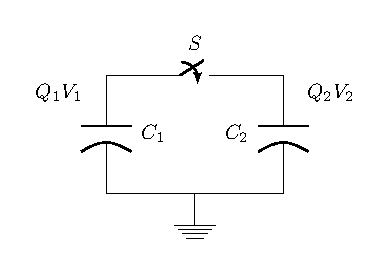
\includegraphics[scale=1.4]{Imagenes/delta_Dirac_03.eps}
    \caption{Circuito eléctrico antes de cerrar el interruptor.}
    \label{fig_figura_delta_Dirac_03}
\end{figure}

% \section{Distribuciones.}

% Las ideas que nos permitieron desarrollar el concepto de la delta de Dirac previamente, se pueden sistematizar en lo que se conoce como \emph{la teoría de distribuciones o funciones generalizadas}.
% \par
% Las funciones generalizadas fueron introducidas en 1935 por el matemático ruso, Sergei Lvóvich Sóbolev (1908 - 1989). De manera independientemente a finales de la década de 1940, el matemático francés, Laurent Schwartz (1915 - 2002) formalizó la teoría de distribuciones, lo que le valió la Medalla Fields en 1950 (que no recibió durante la entrega ya que se le negó la visa para ingresar a los Estados Unidos.)
% \par
% Como el nombre lo sugiere, la teoría tiene como objetivo  \emph{extender la definición de una función}, de manera tal que conceptos como el de la delta de Dirac $\delta (x)$ cuenten con una base matemática firme. En particular la teoría permite extender el concepto de derivada a todas las funciones localmente integrables y a entes aún más generales. Existen varias formas de presentar la teoría de distribuciones, se dará una breve introducción utilizando las integrales de secuencias de funciones del tipo
% \begin{equation}
% \int f_{n}(x) \: g(x) \dd{x} \hspace{1cm} n = 1, 2, 3 , \ldots
% \label{eq:ecuacion_1_99}
% \end{equation}
% Para ello es necesario introducir tres conceptos:
% \begin{enumerate}
% \item El concepto de función de prueba.
% \item El concepto de función admisible.
% \item El concepto de convergencia débil.
% \end{enumerate}
% Hemos visto que una secuencia de funciones $f_{n}(x)$ tal como la secuencia delta de funciones, definida en \ref{secuencias_delta}, nos lleva al concepto matemático de \enquote{función} delta, si la secuencia de integrales converge para funciones apropiadas $g(x)$. Pero ¿Qué quiere decir que sean apropiadas? En la sección anterior vimos que si queremos definir conceptos tales como las derivadas de la función delta, entonces las funciones $g(x)$ deben ser diferenciables. Para definir las derivadas también hemos visto que al integrar por partes, para que las derivadas totales no contribuyan, es necesario que la función $g(x)$ tenga un comportamiento apropiado en infinito. Definimos entonces las funciones $g(x)$ como
% \begin{defi}
% Funciones de prueba.
% Decimos que las función $g(x)$ en la ec. (\ref{eq:ecuacion_1_99}), es de prueba, si es infinitamente diferenciable (clase $C^{\infty}$) y es idénticamente cero fuera de algún intervalo $(a, b)$ (en general este intervalo es diferente para funciones $g(x)$ diferentes).
% \end{defi}
% El nombre de funciones de prueba es adecuado, dado que por ejemplo, la propiedad de filtro de las secuencias delta, se prueba sobre estas funciones. Habiendo definido las funciones de prueba, podemos ahora definir las funciones admisibles (de las cuales seleccionaremos las funciones $f_{n}(x)$ y la convergencia débil.
% \begin{defi}
% Funciones admisibles.

% Decimos que las funciones $f_{n}(x)$ en la ec. (\ref{eq:ecuacion_1_99}) son admisibles, si son infinitamente diferenciables. Su comportamiento en infinito puede ser arbitrario.
% \end{defi}
% \begin{defi}
% Convergencia débil.

% Consideremos una secuencia de funciones admisibles $f_{n}(x)$ con \\ $n = 1, 2, 3, \ldots$
% Decimos que esta secuencia es débilmente convergente si el límite
% \begin{equation}
% \lim_{n \to \infty} \int_{-\infty}^{\infty} f_{n}(x) \:  g(x) \, \dd{x}
% \label{eq:ecuacion_1_100}
% \end{equation}
% existe para todas las funciones de prueba $g(x)$.
% \end{defi}
% Una secuencia débilmente convergente puede o no puede converger en alguno de los sentidos de convergencia usual, como convergencia puntual.
% \par
% Podemos presentar ahora una definición rigurosa de una distribución de la siguiente manera:
% \begin{defi}
% Distribuciones.

% Una distribución $\varphi (x)$ es un concepto matemático asociado con una secuencia débilmente convergente de funciones admisibles para la cual la integral simbólica
% \begin{equation}
% \int_{-\infty}^{\infty} \phi (x) \:  g(x) \, \dd{x}
% \label{eq:ecuacion_1_101}
% \end{equation}
% tiene un significado preciso, por medio de la prescripción
% \begin{equation}
% \int_{-\infty}^{\infty} \phi (x) \: g(x) \, dx = \lim_{n \to \infty} f_{n}(x) \: g(x) \, \dd{x}
% \label{eq:ecuacion_1_102}
% \end{equation}
% \end{defi}

\section{La delta de Dirac.}

Informalmente la delta de Dirac es una \enquote{función} que representa un pico infinitamente agudo expresado simbólicamente por
\begin{align}
\delta (x) = \begin{cases}
0 & x \neq 0 \\
\infty & x = 0
\end{cases}
\label{eq:ecuacion_delta_01}
\end{align}

pero tal que la integral de $\delta (x)$ está normalizada a la unidad:
\begin{align}
\int_{-\infty}^{\infty} \delta (x) \: \dd{x} = 1 
\label{eq:ecuacion_delta_02}
\end{align}

\subsection{Propiedad de filtro.}

La delta de Dirac satisface la siguiente propiedad:
\begin{align}
\int_{-\infty}^{\infty} \delta (x) \: f(x) \: \dd{x} = f(0)
\label{eq:ecuacion_delta_03}
\end{align}

donde $f(x)$ es una función continua.
\par
Esta integral puede ser \enquote{evaluada} utilizando siguiente argumento: dado que $\delta (x) = 0$
para $x \neq 0$, podemos cambiar los límites de integración en la ecuación (\ref{eq:ecuacion_delta_03}) a $- \epsilon$ y $+ \epsilon$, donde $\epsilon$ es un número positivo infinitesimal. Más aún, dado que $f(x)$ es continua en $x = 0$, sus valores dentro del intervalo $( - \epsilon, + \epsilon)$ no diferirán mucho de $f(0)$ y podemos hacer la siguiente aproximación
\begin{align*}
\int_{-\infty}^{\infty} \delta (x) \: f(x) \: \dd{x} = \int_{-\epsilon}^{\epsilon} \delta (x) \: f(x) \: \dd{x} \approx f(0) \int_{-\infty}^{\infty} \delta (x) \: \dd{x}
\end{align*}

Esta aproximación mejora cuando $\epsilon \to 0$. Pero
\begin{align*}
\int_{-\epsilon}^{+\epsilon} \delta (x) \, \dd{x} = 1
\end{align*}

para todos los valores de $\epsilon$, por que $\delta (x) = 0$ para $x \neq 0$ y $\delta (x)$ está normalizada. Así en el límite $\epsilon \to 0$, se tiene
\begin{align*}
\int_{-\infty}^{\infty} \delta (x) \: f(x) \: \dd{x} = f(0)
\end{align*}

\textbf{Nota: } Los límites $-\infty$ y $+\infty$ se pueden reemplazar por cualesquiera números $a$ y $b$, tales que $a < 0 < b$.
\par
Esta integral se le conoce también como \emph{propiedad de filtro} de la función delta, ya que $\delta (x)$ actúa como un filtro, seleccionando de todos los posibles valores de $f(x)$ su valor en el punto $x=0$.

\subsection{Secuencias delta.}\label{secuencias_delta}

La afirmación de que la función $\delta (x)$ está dada por la expresión (\ref{eq:ecuacion_delta_01}) \textit{no es una afirmación apropiada y no se puede utilizar para definir una función}, mucho menos para una función integrable. Una posible definición alterna, podría ser el definir la función $\delta (x)$ como la función que satisface la propiedad de filtro (\ref{eq:ecuacion_delta_03})
\begin{align*}
\int_{-\infty}^{+ \infty} \delta (x) \, f(x) \, \dd{x} = f(0)
\end{align*}

para toda función continua $f(x)$. Sin embargo es posible demostrar que no existe ninguna función con esa propiedad. Por lo que 
\begin{center}
\textit{¡¡la función delta no es una función en el sentido matemático usual!!}
\end{center}

¿Qué se hace entonces?  ¿Dirac nos engañó con su propuesta? Lo que sucede es que existen secuencias de funciones de pico pronunciado, las cuales en el límite en que el pico es infinitamente delgado e infinitamente alto, satisfacen la propiedad de filtro.
\par
La siguiente puede ser una secuencia $\phi_{n} (x)$ con $n = 1, 2, 3, \ldots$, tal que
\begin{align*}
\lim_{n \to \infty} \int_{-\infty}^{+ \infty} \phi_{n}(x) \, f(x) \dd{x} =  f(0)
\end{align*}

\begin{defi}
Llamamos secuencias delta $\delta_{n} (x)$ a una secuencia de funciones de pico pronunciado, que satisfacen
\begin{align*}
\lim_{n \to \infty} \int_{-\infty}^{+ \infty} \phi_{n} (x) \: f(x) \: \dd{x} =  f(0)
\end{align*}
\end{defi}

\begin{ejemplo}
La secuencia de funciones
\begin{align}
\phi_{n} (x) = \begin{cases}
0 & x < - \dfrac{1}{2 \, n} \\
n & - \dfrac{1}{2 \, n} < x < \dfrac{1}{2 \, n} \\
0 & 0 >  \dfrac{1}{2 \, n}
\end{cases}
\hspace{1cm} n = 1, 2, 3, \ldots
\label{eq:ecuacion_delta_04}
\end{align}

es una secuencia delta.
\end{ejemplo}
\begin{figure}[H]
    \centering
    \includestandalone{Figuras/plot_secuencia_delta}
    \caption{Secuencia delta para valores de $n=1,2,\ldots,10$. El área debajo de la curva para cada $\phi_{n}$ siempre vale $1$.}
    \label{fig:secuncia_delta_01}
\end{figure}

Para verificar esta afirmación consideremos la integral
%Apuntes FETI página 46
\begin{align*}
\int_{-\infty}^{\infty} \phi_{n} (x) \, f(x) \dd{x}
\end{align*}

para cualquier función continua arbitraria $f(x)$. De la expresión (\ref{eq:ecuacion_delta_04}) para la secuencia delta se tiene
\begin{align*}
\int_{-\infty}^{+ \infty} \phi_{n} (x) \, f(x) \dd{x} = \int_{-\frac{1}{2 \, n}}^{\frac{1}{2 \, n}} n \, f(x) \, \dd{x} = n \int_{-\frac{1}{2 \, n}}^{\frac{1}{2 \, n}} f(x) \,  \dd{x}
\end{align*}

Utilizando el teorema del valor medio para integrales, podemos deducir que
\begin{align*}
n \int_{-\frac{1}{2 \, n}}^{\frac{1}{2 \, n}} f(x) \dd{x} = n \, \dfrac{1}{n} f(\xi) = f(\xi), \hspace{1cm} - \dfrac{1}{2 \, n} \leq \xi \leq \dfrac{1}{2 \, n}
\end{align*}

En el límite cuando $n \to \infty$, $\xi \to 0$. De la continuidad de la función $f(x)$ se sigue que $f(\xi) \to f(0)$, obteniendo así el resultado
\begin{align*}
\lim_{n \to \infty} \int_{-\infty}^{+ \infty} \: \phi_{n}(x) \: f(x) \: \dd{x} = f(0)
\end{align*}

lo que nos dice que la secuencia (\ref{eq:ecuacion_delta_04}) es una secuencia delta.
\par
Nótese que la secuencia delta (\ref{eq:ecuacion_delta_04}) no es derivable en el punto $x = 0$. Para muchos propósitos es deseable
construir secuencias delta de funciones que sean continuas y diferenciables. Por ejemplo, en las figuras (\ref{fig:plot_secuencia_01}), (\ref{fig:plot_secuencia_02}) y (\ref{fig:plot_secuencia_03}) podemos apreciar algunas secuencias delta con estas características:

\begin{figure}[H]
    \centering
    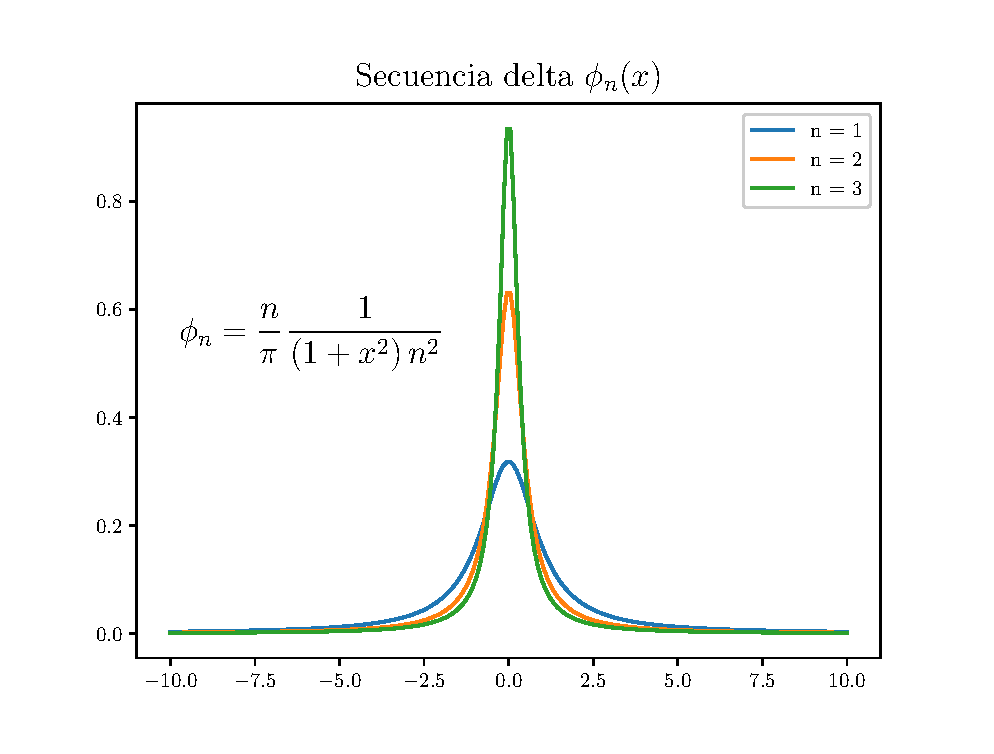
\includegraphics[scale=0.8]{Imagenes/secuencia_delta_01.eps}
    \caption{Secuencia para $\phi_{n}$ con $n=1,2,3$}
    \label{fig:plot_secuencia_01}
\end{figure}


\begin{figure}[H]
    \centering
    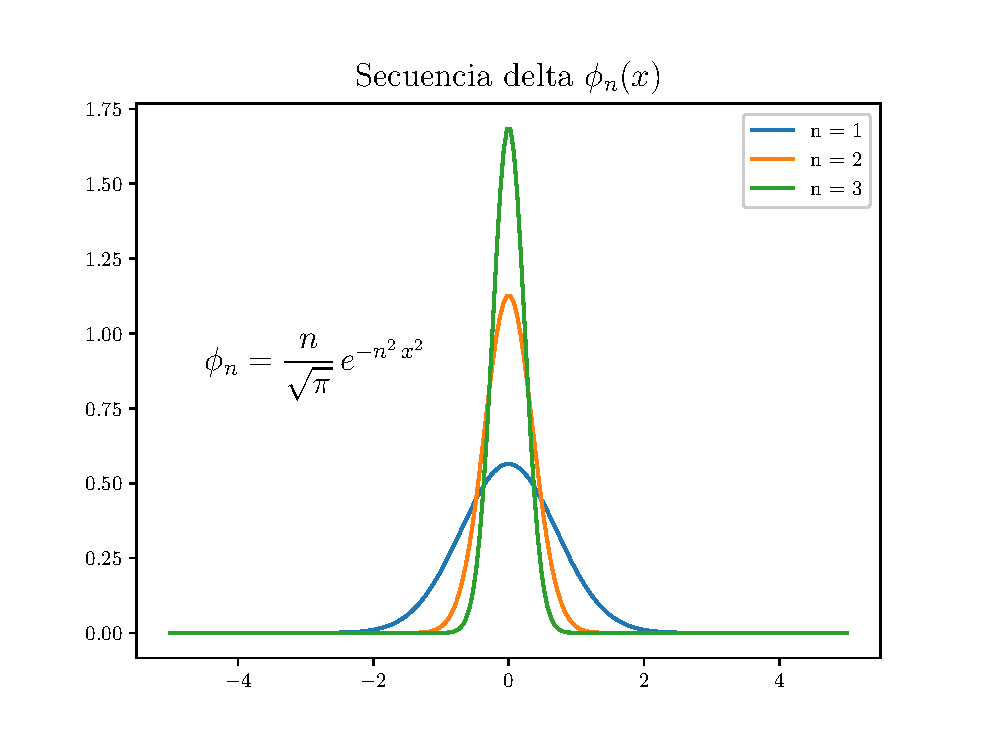
\includegraphics[scale=0.8]{Imagenes/secuencia_delta_02.eps}
    \caption{Secuencia para $\phi_{n}$ con una función exponencial.}
    \label{fig:plot_secuencia_02}
\end{figure}

\begin{figure}[H]
    \centering
    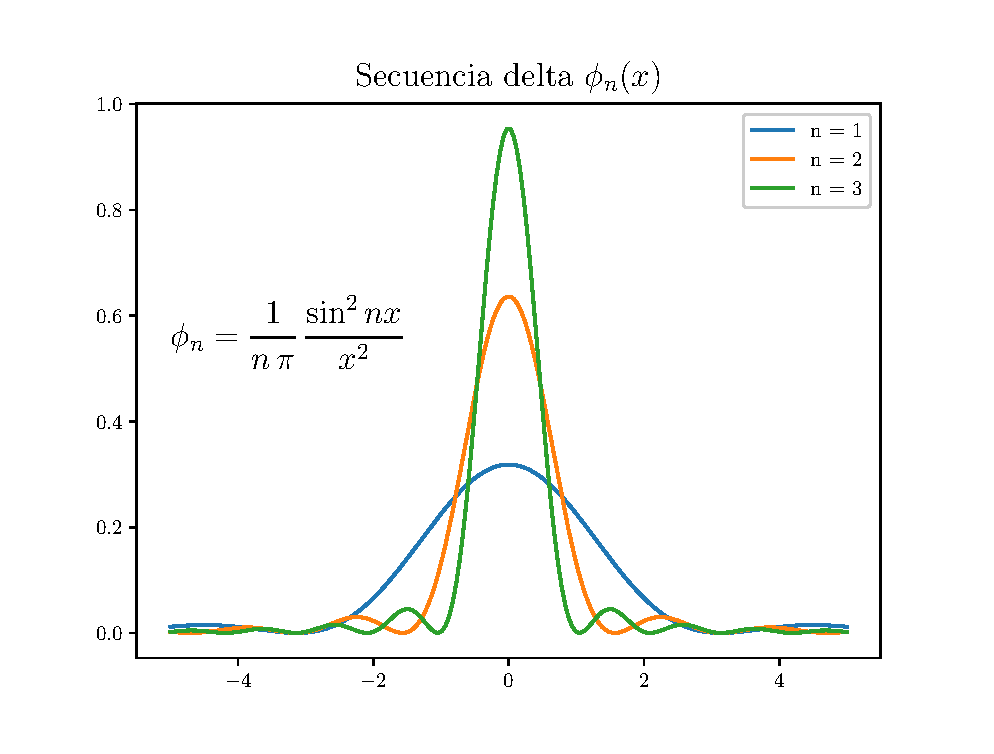
\includegraphics[scale=0.8]{Imagenes/secuencia_delta_03.eps}
    \caption{Secuencia para $\phi_{n}$ con una función $\sin^{2}(x)/x$}
    \label{fig:plot_secuencia_03}
\end{figure}

Tomemos en cuenta que no es correcto expresar que éstas secuencias convergen a la función delta: los límites de esas secuencias \emph{no existen} (de acuerdo a las definiciones conocidas de convergencia).

Todas estas funciones están normalizadas a la unidad
\begin{equation}
\lim_{n \to \infty} \int_{- \infty}^{+ \infty} \phi_{n}(x) \: \dd{x} = 1
\label{eq:ecuacion_delta_05}
\end{equation}

\subsection{Propiedades de la delta de Dirac.}

Una vez que hemos definido la delta de Dirac, nos gustaría saber ahora como operar con y en ella. ¿Es posible decir algo sobre su derivada? La respuesta a esta pregunta es afirmativa y las secuencias delta hechas de funciones diferenciables nos permiten responder a la pregunta de manera precisa.
\par
Por ejemplo, sea la secuencia delta
\begin{align*}
\phi_{n} &= \dfrac{n}{\sqrt{\pi}} e^{-n^{2} x^{2}}
\end{align*}

entonces, al diferenciar la secuencia
\begin{align*}
\dv{\phi_{n}(x)}{x} = - \dfrac{2 \: n^{3}}{\sqrt{\pi}} \: x \: \exp(-n^{2} \: x^{2})
\end{align*}

\begin{figure}[H]
    \centering
    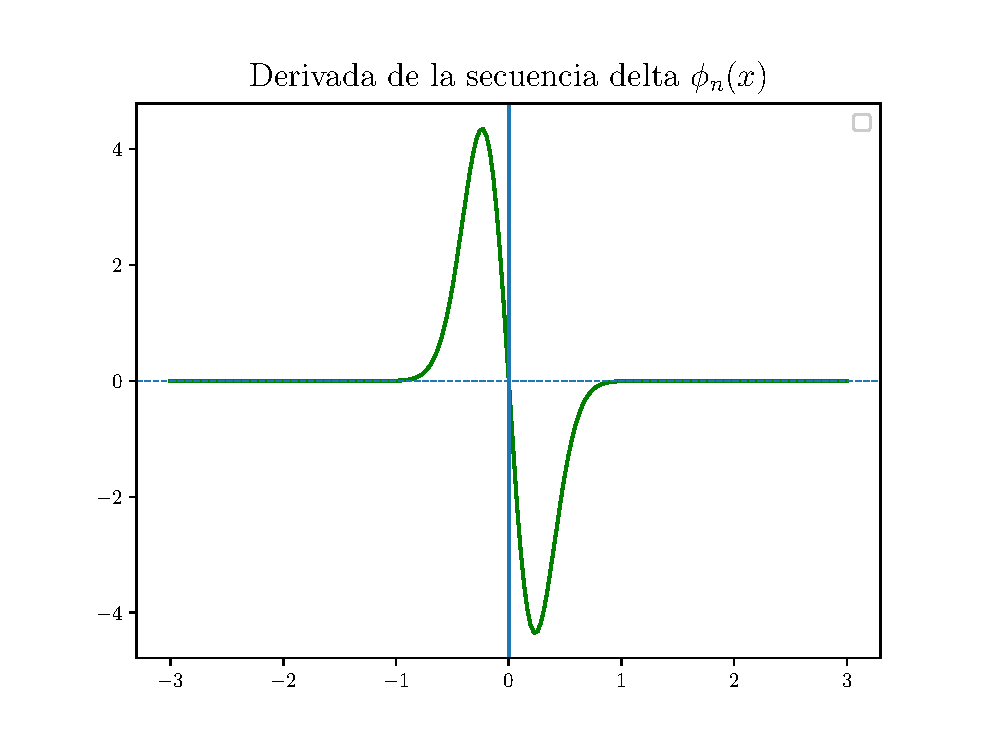
\includegraphics[scale=0.8]{Imagenes/secuencia_delta_04.eps}
    \caption{Derivada de la secuencia delta.}
    \label{fig:fig_figura_delta_04}
\end{figure}

Consideremos ahora la integral
\begin{align*}
\int_{-\infty}^{+\infty} \dv{\phi_{n}(x)}{x} \: f(x) \dd{x}
\end{align*}

donde $f(x)$ es diferenciable. Integrando por partes, se obtiene
\begin{align*}
\int_{-\infty}^{+\infty} \dv{\phi_{n}(x)}{x} \: f(x) \dd{x} = \phi_{n} \: f(x) \eval_{-\infty}^{+\infty} - \int_{-\infty}^{+\infty} \phi_{n} \: \dv{f(x)}{x} \dd{x}
\end{align*}
Suponemos que
\begin{align*}
\lim_{n \to \infty} \left( \dfrac{n}{\sqrt{\pi}} \right) \exp(-n^{2} \, x^{2}) \, f(x) = 0
\end{align*}

Esto normalmente es cierto, ya que estamos considerando funciones para las cuales la integral
\begin{align*}
\int_{-\infty}^{+\infty} \phi_{n}(x) \, f(x) \dd{x} 
\end{align*}

converge.
\par
Entonces, haciendo que $n \to \infty$, tenemos
\begin{align*}
\lim_{n \to \infty} \int_{-\infty}^{+\infty} \dv{\phi_{n}(x)}{x} \: f(x) \dd{x} = - \lim_{n \to \infty} \phi_{n}(x) \: \ptilde{f} (x) \dd{x} =  - \ptilde{f}(0)
\end{align*}

Vemos entonces que la secuencia $\ptilde{\phi}(x)$ está relacionada con la propiedad de filtro.

\begin{propiedad}
Propiedad de filtro de las derivadas.
\\
La delta de Dirac satisface la siguiente propiedad:
\begin{align*}
\int_{-\infty}^{+\infty} \dv{\delta(x)}{x} \, f(x) \, \dd{x} = - \dv{f(0)}{x}
\end{align*}

con $f(x)$ una función diferenciable.
\par
Con la idea anterior, se presenta la propiedad para las derivadas de orden superior de $\delta (x)$:
\begin{align*}
\int_{-\infty}^{+\infty} \dv[m]{\delta (x)}{x} \, f(x) \dd{x} =  (-1)^{m} \, \dv[m]{f(0)}{x}
\end{align*}

Es necesario enfatizar que la expresión anterior tiene significado sólo cuando asumimos directamente que las funciones involucradas son $m$ veces diferenciables y que las integrales
\begin{align*}
\int_{-\infty}^{+\infty} \dv[k]{\phi_{n}(x)}{x} \, f(x) \dd{x}
\end{align*}

convergen para todo valor de $n$ y para todo valor de $k$ de $0$ a $m$.
\end{propiedad}

La delta de Dirac satisface varias propiedades y conocerlas es de mucha utilidad cuando resolvemos problemas específicos en física. 
\par

\begin{propiedad}
Para el producto de la delta de Dirac con una función se tiene que
\begin{align}
x \: \delta(x) &= 0 \\[0.5em]
f(x) \: \delta(x - a) &= f(a) \: \delta(x - a)
\end{align}
\end{propiedad}

\begin{propiedad}
La paridad de la delta de Dirac y su derivada es
\begin{align}
\delta (-x) &= \delta (x) \\[0.5em]
\ptilde{\delta} (-x) &= - \ptilde{\delta} (x)
\end{align}

\end{propiedad}

\begin{propiedad}
También satisface las relaciones
\begin{align}
\delta(a \, x) &= \dfrac{1}{\abs{a}} \, \delta (x), \hspace{1cm} a \neq 0 \\[0.5em]
\delta (x^{2} - a^{2}) &= \dfrac{1}{2 \, a} \big[ \delta (x + a) + \delta (x - a) \big] \hspace{1cm} a > 0
\end{align}
\end{propiedad}

\begin{propiedad}
Las propiedades de filtro
\begin{align}
\int_{-\infty}^{\infty} f(x) \, \delta (x - a) \, \dd{x} &= f(a) \\[0.5em]
\int \delta (a - x) \, \delta (x - b) \, \dd{x} &= \delta (a - b)
\end{align}

\end{propiedad}

\section{Introduciendo más variables.}

Al introducir más variables:
\begin{align}
\delta (\va{\bm{r}} - \va{\bm{r_{0}}}) = \delta (x - x_{0}) \, \delta (y - y_{0}) \, \delta (z - z_{0})
\label{eq:ecuacion_A_03}
\end{align}

de manera que al integrar sobre todo el espacio tenemos:
\begin{align*}
\int \delta (\va{\bm{r}} - \va{\bm{r_{0}}}) \, \dd{x} \dd{y}  \dd{z} = 1
\end{align*}

\textbf{Ejemplo:}

La función delta permite especificar la densidad de carga debida a un conjunto de $N$ cargas puntuales de valores $q_{i}$ situadas en posiciones $\va{r_{i}}$  como:
\begin{align}
\rho (\va{r}) = \sum_{i=1}^{N} q_{i} \, \delta(\va{r} - \va{r_{i}})
\label{eq:ecuacion_A_04}
\end{align}

Las propiedades de la función delta permiten obtener el potencial $\varphi(\va{r})$ evaluando la función dentro de la integral en los puntos $\va{r_{i}}$, es decir:
\begin{align}
\varphi(\va{r}) = \int \dfrac{\rho(\va{\ptilde{r}})}{\abs{\va{r} - \va{\ptilde{r}}}} \: d^{3}\ptilde{r} = \sum_{i=1}^{N} q_{i} \int \dfrac{\delta ( \va{r} - \va{r_{i}})}{\abs{\va{r} - \va{\ptilde{r}}}} \: d^{3}\ptilde{r} = \sum_{i=1}^{N} \dfrac{q_{i}}{\abs{\va{r} - \va{r_{i}}}}
\label{eq:ecuacion_A_05}
\end{align}

Nótese que $\delta (x)$ tiene unidades de inverso de $x$ y $\delta (\va{r})$ tiene unidades de densidad numérica.
\par
La función $\delta$ toma una forma particular en coordenadas cilíndricas y esféricas, dadas por la condición de normalización:
\begin{enumerate}
\item Para coordenadas cilíndricas
\begin{equation}
\int \delta (\va{r} - \va{r}_{0}) \: R \: \dd{R} \: \dd{\varphi} \: \dd{z} \Rightarrow \delta (\va{r}) =  \dfrac{1}{R} \: \delta (R - R_{0}) \: \delta (\varphi - \varphi_{0}) \: \delta (z - z_{0})
\end{equation}
\item  Para coordenadas esféricas
\begin{equation}
\begin{aligned}
\int & \delta (\va{r} - \va{r}_{0}) \: r^{2} \, \dd{r} \, \sin \theta \, \dd{\theta} \, \dd{\varphi} = 1 \\
&\Rightarrow \delta (\va{r}) = \dfrac{1}{r^{2}} \: \delta (r - r_{0}) \, \delta (\cos \theta - \cos \theta_{0}) \, \delta (\varphi - \varphi_{0})
\end{aligned}
\end{equation}
\end{enumerate}

A continuación se indican algunas funciones que en el límite generan la función delta:
\begin{align*}
\delta(x) = \begin{cases}
\displaystyle
\lim_{\varepsilon \to 0^{+}} \dfrac{1}{\pi} \, \dfrac{\varepsilon}{x^{2} + \varepsilon^{2}} & \mbox{Lorentz} \\[1.5em]
\displaystyle
\lim_{\sigma \to 0^{+}} \dfrac{1}{\sigma \, \sqrt{2 \, \pi}} \, \exp \left( - \dfrac{x^{2}}{2 \, \sigma^{2}} \right) & \mbox{Gaussiana} \\[1.5em]
\displaystyle \lim_{\varepsilon \to 0^{+}} \dfrac{\sin(x / \varepsilon)}{ \pi \, x} & \mbox{Dirichlet} \\[1.5em]
\displaystyle \lim_{L \to \infty} \dfrac{1}{2 \, \pi} \int_{- \abs{L}}^{\abs{L}} \exp(i \, k \, x) \dd{k} & \mbox{Fourier}
\end{cases}
\end{align*}

\end{document}